\documentclass[10pt,a4paper]{article}
\usepackage[margin=2.2cm]{geometry}
\usepackage{fontspec}
\usepackage{kotex}
\setmainfont{Apple SD Gothic Neo}
\setsansfont{Apple SD Gothic Neo}
\usepackage{amsmath,amssymb}
\usepackage{graphicx}
\usepackage{booktabs}
\usepackage{caption}
\usepackage[dvipsnames]{xcolor}
\usepackage[colorlinks=true,linkcolor=MidnightBlue,citecolor=MidnightBlue,
            urlcolor=MidnightBlue]{hyperref}
\usepackage{titlesec}
\titleformat{\section}{\large\bfseries}{\thesection}{0.6em}{}
\titleformat{\subsection}{\normalsize\bfseries}{\thesubsection}{0.5em}{}
\captionsetup{font=small,labelfont=bf}
\setlength{\parskip}{0.35em}
\setlength{\parindent}{0pt}

\usepackage{mdframed}
\newmdenv[linewidth=0.4pt,linecolor=gray!60,backgroundcolor=gray!5,
          innertopmargin=6pt,innerbottommargin=6pt,skipabove=8pt,skipbelow=8pt]{claimbox}
\newcommand{\claim}[2]{\begin{claimbox}\textbf{주장.} #1\par\smallskip
  \textcolor{gray!70}{\textbf{반증 조건.} #2}\end{claimbox}}

\title{\bfseries 시간이 아니라 진폭이 가른다\\[2pt]
\large 곡선 겹침 시험 --- 그리고 다섯 번째 갈래 충돌은 내 규약 위반이다}
\author{월드모델 실험실 · 노트 $813$}
\date{2026-08-07}
\begin{document}\maketitle

\section{한 줄}

사용자의 인수분해 가설 --- \emph{장 $=$ 공유 형태 $\times$ 도메인 모수(시간
스케일 · 진폭)} --- 을 wiki\_after $2{,}137$곡선으로 쟀다(노트 $790$ 과 다른
물음이다: 그건 감쇠율$\to$라벨 사상의 전이였고 이건 \textbf{곡선 모양 자체}다).

\begin{center}
\begin{tabular}{lrrr}
\toprule
& $\tau$(일) & 진폭(log1p) & 자기-반쪽 RMSE \\
\midrule
게임 & $14$ & $\mathbf{1.828}$ & $\mathbf{0.028}$ \\
세계애니 & $3$ & $\mathbf{1.155}$ & $\mathbf{0.018}$ \\
시장팝업 & $20$ & $0.475$ & $0.260$ \\
모바일 & $10$ & $0.374$ & $0.134$ \\
웹툰 & $2$ & $0.305$ & $0.239$ \\
애니 & $15$ & $0.173$ & $\mathbf{0.475}$ \\
\bottomrule
\end{tabular}
\end{center}

시간 정규화는 교차 RMSE 를 $\mathbf{5.4\%}$ 밖에 못 줄인다($0.331 \to 0.313$)
--- \textbf{시간 스케일은 주 분리자가 아니다.} 가르는 것은 \textbf{진폭}이다:
진폭 큰 둘은 곡선이 실재하고(자기 반쪽과 정확히 겹침), 작은 넷은 \textbf{자기
자신과도 안 겹친다.}

\begin{figure}[t]\centering
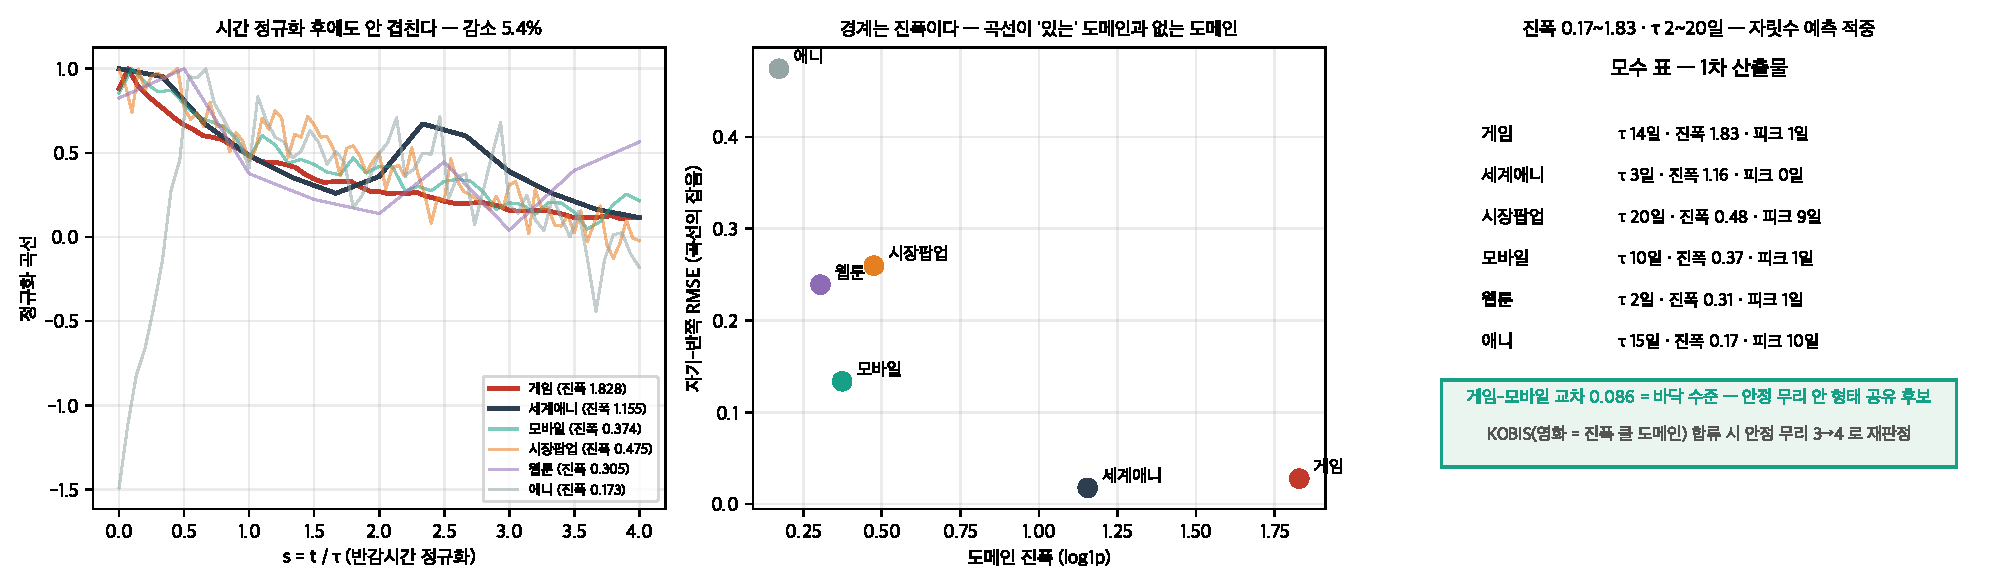
\includegraphics[width=0.99\textwidth]{figs/amp.pdf}
\caption{왼쪽: 정규화 후에도 안 겹치는 곡선들. 가운데: \textbf{진폭 대 자기-잡음}
--- 경계가 보인다. 오른쪽: 모수 표와 남는 후보.}
\end{figure}

\section{실질 발견 셋}

\claim{\textbf{① ``곡선이 있는 도메인''과 ``없는 도메인''의 구분이 형태 비교보다
먼저다.} 애니(진폭 $0.173$)의 교차 RMSE($0.57{\sim}0.61$)는 애니 자기
바닥($0.475$)과 같은 자리다 --- 주의 임펄스가 잡음 수준이면 ``평균 곡선''이
안정된 대상이 아니고, 그 도메인을 형태 비교에 넣는 것 자체가 범주 오류다.
\textbf{② 안정 무리 안에서는 겹침이 실재 후보다} --- 게임-모바일 $0.086$ 은 바닥
수준이다. \textbf{③ 모수 표가 1차 산출물이다}($\tau$ $2{\sim}20$일 · 진폭
$0.17{\sim}1.83$ --- 자릿수 차이 예측 적중).}
{안정 무리가 둘$+$반(게임·세계애니·모바일)뿐이라 ``형태 공유''는 아직 판정이
아니라 후보다. \textbf{KOBIS(영화 --- 주의 임펄스가 클 도메인)가 합류하면 안정
무리가 셋$\to$넷이 되어 판정력이 선다} --- 수집 우선순위의 또 하나의 근거.}

\section{다섯 번째 갈래 충돌 --- 이번 것은 규약 위반이다}

(좋) ``교차 $\leq 2\times$바닥''($0.313 \leq 0.384$ 참)과 (해) ``감소
$<10\%$''($5.4\%$ 참)가 \textbf{동시에 참}이었다. 바닥이 불안정 도메인들
때문에 부풀어 (좋)의 조건이 헐거워진 것이다.

\claim{\textbf{규약 $46$(배타 갈래엔 우선순위)을 세워 놓고 내가 안 지켰다} ---
갈래 상호작용 계열의 다섯 번째이고, 규약이 있는데 어긴 첫 사례다. 판정문 없이
실질만 기록했고(승격·채택이 걸린 측정이 아니라 가능한 처분), 다음 사전등록부터
\textbf{갈래에 번호 우선순위를 강제}한다.}
{규약이 있어도 어기는 것은 규약이 산문이라서다 --- `check` 가 사전등록의 갈래
구조까지 검사하게 만들 수 있는지가 남은 물음이고, 그것은 사전등록을 산문이
아니라 \textbf{구조화된 형식}으로 옮기는 일이다. 비용이 커서 미결로만 적는다.}

\end{document}
